\documentclass[12pt,a4paper,openright,twoside]{book}
\usepackage[utf8]{inputenc}
\usepackage{disi-thesis}
\usepackage{code-lstlistings}
\usepackage{notes}
\usepackage{shortcuts}
\usepackage{acronym}

\school{\unibo}
\programme{Corso di Laurea in Ingegneria e Scienze Informatiche}
\title{Eterogeneità dei sistemi di Aggregate Programming: estensione del sistema ScaFi per l'uso di robot Thymio}
\author{Elvis Perlika}
\date{\today}
\subject{Objective Oriented Programming}
\supervisor{Chiar.mo Prof. Mirko Viroli}
\cosupervisor{Dott. Gianluca Aguzzi}
\session{III}
\academicyear{2023-2024}

% Definition of acronyms
\acrodef{IoT}{Internet of Thing}
\acrodef{vm}[VM]{Virtual Machine}


\mainlinespacing{1.241} % line spacing in mainmatter, comment to default (1)

\begin{document}

\frontmatter\frontispiece

\begin{abstract}	
Max 2000 characters, strict.
\end{abstract}

\begin{dedication} % this is optional
    Qualsiasi tecnologia sufficientemente avanzata è indistinguibile dalla magia. \\ Terza Legge di Arthur C. Clarke
\end{dedication}

%----------------------------------------------------------------------------------------
\tableofcontents   
\listoffigures     % (optional) comment if empty
\lstlistoflistings % (optional) comment if empty
%----------------------------------------------------------------------------------------

\mainmatter

%----------------------------------------------------------------------------------------
\chapter{Introduction}
\label{chap:introduction}
%----------------------------------------------------------------------------------------

Write your intro here.
\sidenote{Add sidenotes in this way. They are named after the author of the thesis}

You can use acronyms that your defined previously,
such as \ac{IoT}.
%
If you use acronyms twice,
they will be written in full only once
(indeed, you can mention the \ac{IoT} now without it being fully explained).
%
In some cases, you may need a plural form of the acronym.
%
For instance,
that you are discussing \acp{vm},
you may need both \ac{vm} and \acp{vm}.

\paragraph{Structure of the Thesis}

\note{At the end, describe the structure of the paper}

%----------------------------------------------------------------------------------------
\chapter{Background}
\label{chap:background}
%----------------------------------------------------------------------------------------

I suggest referencing stuff as follows: \cref{fig:random-image} or \Cref{fig:random-image}

% \begin{figure}
%     \centering
%     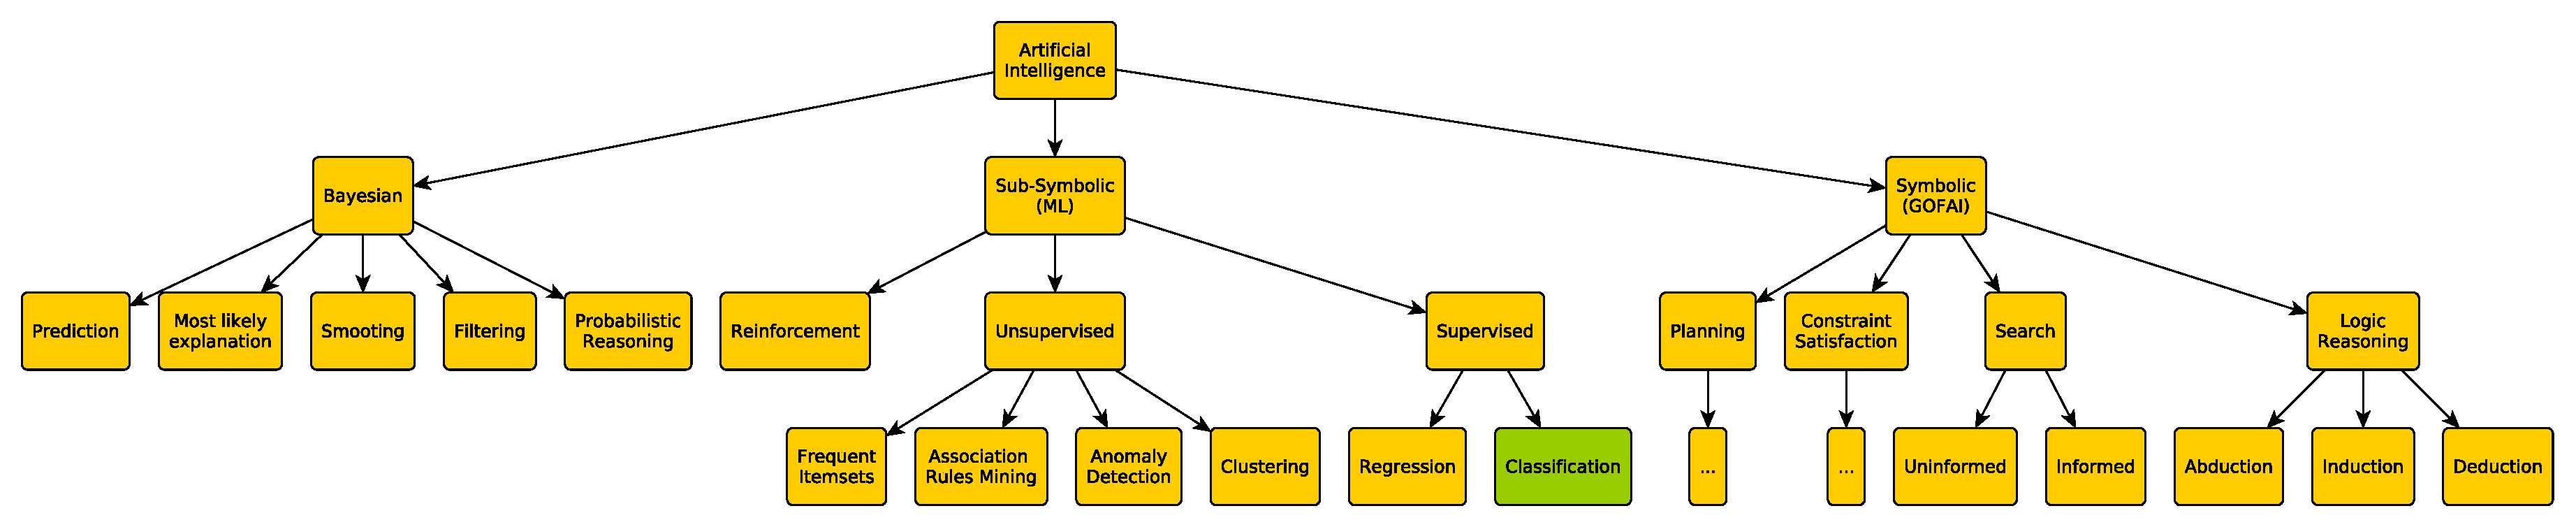
\includegraphics[width=.8\linewidth]{figures/random-image.pdf}
%     \caption{Some random image}
%     \label{fig:random-image}
% \end{figure}

\section{Paradigma OOP e Programmazione Funzionale}

\subsection{Paradigma OOP}

L'Objective Oriented Programming è un paradigma nel senso stretto del termine poichè rappresenta un modo di organizzare e rappresentare un mondo. Il paradigma in questione deve la sua potenza nella capacità di simulare entità reali. 
È rilevante parlare di OOP in quanto il paradigma di programmazione funzionale, che è alla base di ScaFi, è un'estensione di esso. 
Il potere della programmazione ad Oggetti (OOP), come detto precedentemente, risiede nella capacità di simulare un mondo e permette di farlo grazie agli "oggetti", essi sono istanze di Classi, le quali a loro volta sono strutture dati astratte che permettono ad ogni loro istanza di avere uno stato (definito dai \textit{fields}) e un comportamento (definito dai \textit{methods}).
I pilastri della programmazione ad oggetti sono l'incapsulamento, l'ereditarietà e il polimorfismo\cref{fig:OOP}.

\begin{figure}
    \centering
    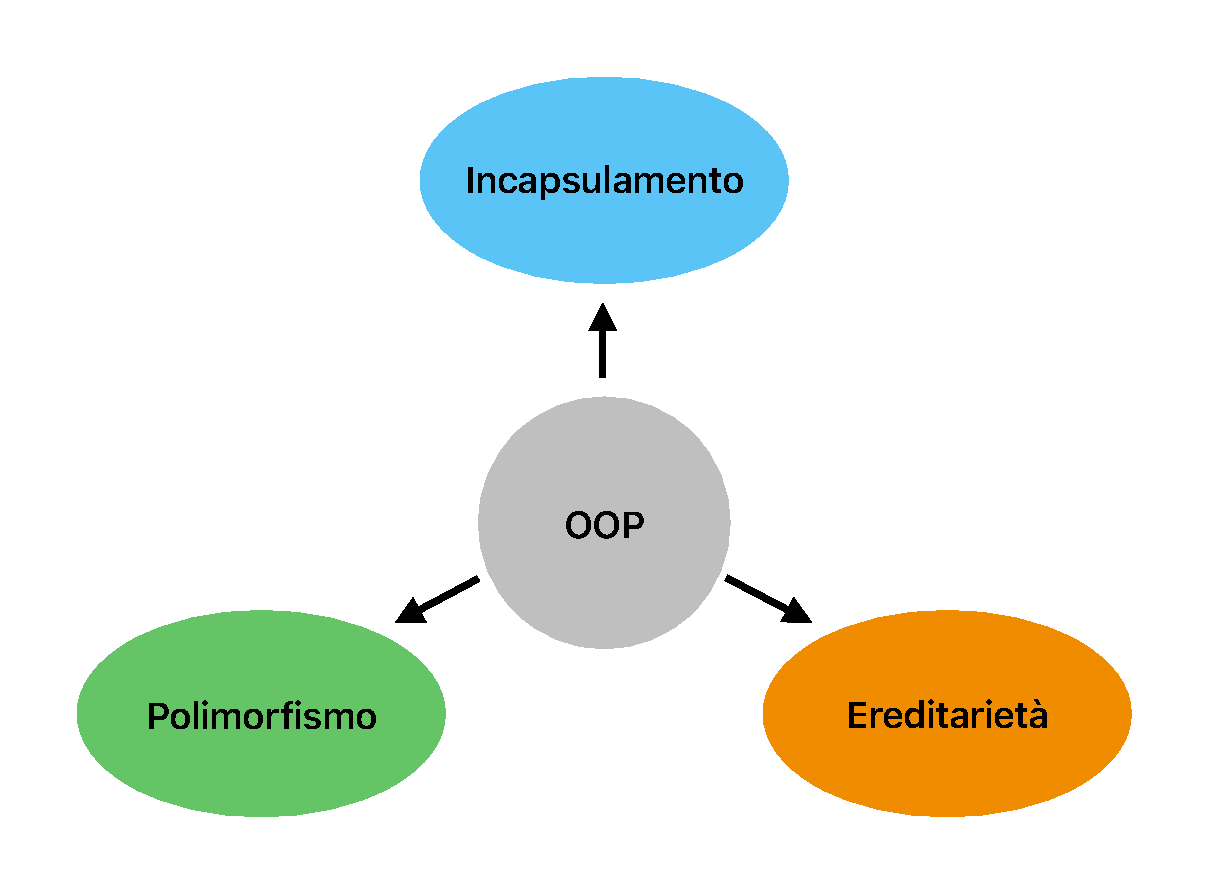
\includegraphics[width=.6\linewidth]{figures/OOP.pdf}
    \caption{Principi della OOP}
    \label{fig:OOP}
\end{figure}

\begin{itemize}
    \item \textbf{Incapsulamento}: Questo principio vuole che i dettagli implementativi di una classe siano nascosti ad altre classi. È un approccio progettuale che mira ad isolare ogni sistema e set di dati. 
    \item \textbf{Ereditarietà}: Con ereditarietà si intende la specializzazione di una classe figlia da una classe madre. Questo permette di creare classi più specifiche che ereditano le proprietà e i metodi della classe madre incoraggiando il riuso del codice.
    \item \textbf{Polimorfismo}: Il polimorfismo è la capacità di un ogetto di assumere più forme. In OOP il polimorfismo è realizzato attraverso l'\textit{overloading} e l'\textit{overriding}. L'overloading è la possibilità di avere più metodi con lo stesso nome ma con diversi parametri, mentre l'overriding è la possibilità di ridefinire un metodo della classe madre nella classe figlia.
\end{itemize}

La programmazione ad oggetti si differenzia dalla più clasica programmazione funzionale in quanto controlla la complessità del software supportando la scomposizione gerarchica attraverso sia i dati che l'astrazione procedurale.
Tra i benefici della OOP troviamo la predisposizione al miglioramento della qualità e della leggibilità del codice e la facilità di manutenzione.

Non è, tuttavia, priva di difetti. Questi ultimi sono ciò che la programmazione funzionale risolve parzialmente.

\subsection{Programmazione Funzionale}

\section{Paradigma dell'Aggregate Programming}

\section{ScaFi e Macro-Swarm}

\section{Thymio e tdmclient}

\section{Aruco Tag}

%----------------------------------------------------------------------------------------
\chapter{Analisi}
\label{chap:analisi}
%----------------------------------------------------------------------------------------

\section{Estendibilità del sistema ad un nuovo modello di Robot (Thymio)}

\section{Gestione dei vincoli di compatibilità del sistema Thymio}


%----------------------------------------------------------------------------------------
\chapter{Design}
\label{chap:design}
%----------------------------------------------------------------------------------------

\section{Architettura server Flask}

\section{File di configurazione}

%----------------------------------------------------------------------------------------
\chapter{Implementazione}
\label{chap:implementazione}
%----------------------------------------------------------------------------------------

\section{Implementazione del server Flask}

\section{Esempi di Algoritmi AP applicati ai Robot Wave e Thymio nello stesso ambiente}

You may also put some code snippet (which is NOT float by default), eg: \cref{lst:random-code}.

\lstinputlisting[float,language=Java,label={lst:random-code}]{listings/HelloWorld.java}

\section{Fancy formulas here}

%----------------------------------------------------------------------------------------
\chapter{Conclusione}
\label{chap:conclusione}
%----------------------------------------------------------------------------------------

%----------------------------------------------------------------------------------------
% BIBLIOGRAPHY
%----------------------------------------------------------------------------------------

\backmatter

\nocite{*} % Remove this as soon as you have the first citation

\bibliographystyle{alpha}
\bibliography{bibliography}

\begin{acknowledgements} % this is optional
Optional. Max 1 page.
\end{acknowledgements}

\end{document}
